%\subsection{Code Implementation}\label{ssec:Code}
%\lstinputlisting{example_code.py}

\subsection{Task I: Basic Data Consideration}\label{ssec:task1}
%\begin{multicols}{2}
The data given in the ASCII file contained $ \num{2.5e6} $ points in the trajectory of alanine dipeptide. The trajectory was given as two columns containing the $ \phi $ and $ \psi $ angles respectively:
\begin{equation}\label{eq:phi-psi-range}
	\phi,\psi \in \left[-180\degree,180\degree\right[
\end{equation} 
%
In the task instructions, it was given that the points were separated by $ \Delta t = $\SI{200}{\femto\second}. Since the number of data points, say $ N $, was $ \num{2.5e6} $, the timescale of the entire trajectory could be calculated as
\begin{dmath}\label{eq:t-scale-calc}
	t_{\text{final}} = N\times\Delta t
	= \num{2.5e6}\times \SI{200}{\femto\second}
	= \num{2.5e6}\times 200\times\num{e-15}\unit{\second}
	= \num{5e-7}\unit{\second}
	= \SI{500}{\nano\second}
\end{dmath}
%
After importing the data using the \texttt{read_csv} function in the \texttt{pandas} package and setting the above timescale, the time evolution of the dihedral angles were plotted as shown in figure \ref{fig:dihedralevolution}.
%
\begin{figure*}[htbp]
	\centering
	%	\rule{\linewidth}{3cm}
	\includegraphics[width=\linewidth]{../Coding/plots/dihedral_evolution.pdf}
	\caption{Time evolution of dihedral angles \textcolor{cyan}{$ \phi $} and \textcolor{red!70}{$ \psi $} at different time scales: (A) and (B) in picoseconds, (C) and (D) in fractions of a nanosecond, (E) and (F) in tens of nanoseconds.}
	\label{fig:dihedralevolution}
\end{figure*}
%
Here one can see how the angles evolve on several timescales. Fast oscillatory motions were observed on the picosecond scale \ref{fig:dihedralevolution}(A,B), as well as shifts between different conformational states at nanosecond scale (C,D,E and F). 
%

The circular (and not linear) nature of the given data (equation \ref{eq:phi-psi-range}) gives rise to some problems for analysis. At the stage of basic data visualization, one could already see that a quick viewing of the plot in figure \ref{fig:dihedralevolution} can be misinterpreted. For example, consider the jump from $ \phi_1 \approx -100\degree $ to $ \phi_2 \approx+140\degree $ in the panel E of the figure. For linear data, this jump would mean that the value changes by $\Delta\phi= 140-(-100) = 240 $ units. However, since these are angles, the actual jump\footnote{A function called \texttt{angle_difference} was defined in the Jupyter notebook to calculate the actual difference between two angles.} is only by $ 110\degree $ (see figure \ref{fig:example-circ-data}). %This problem is revisited later in the assignment. 

\begin{figure}[htbp]
	\centering
	%	\tikzset{every picture/.style={line width=0.75pt}} %set default line width to 0.75pt        
	%	
	%	\begin{tikzpicture}[x=0.75pt,y=0.75pt,yscale=-1,xscale=1]
		%		%uncomment if require: \path (0,300); %set diagram left start at 0, and has height of 300
		%		
		%		%Shape: Axis 2D [id:dp8778873795993651] 
		%		\draw [color={rgb, 255:red, 155; green, 155; blue, 155 }  ,draw opacity=1 ] (138.53,123.78) -- (301.73,123.78)(219.92,36) -- (219.92,202.67) (294.73,118.78) -- (301.73,123.78) -- (294.73,128.78) (214.92,43) -- (219.92,36) -- (224.92,43)  ;
		%		%Straight Lines [id:da2729508144276438] 
		%		\draw [color={rgb, 255:red, 139; green, 87; blue, 42 }  ,draw opacity=1 ]   (219.92,123.78) -- (202.93,53.2) ;
		%		%Straight Lines [id:da7165137837483855] 
		%		\draw [color={rgb, 255:red, 126; green, 211; blue, 33 }  ,draw opacity=1 ]   (166.4,168) -- (219.92,123.78) ;
		%		%Shape: Arc [id:dp46003831223859915] 
		%		\draw  [draw opacity=0] (213.96,128.92) .. controls (209.31,125.73) and (207.49,119.11) .. (209.93,113.03) .. controls (211.03,110.3) and (212.82,108.08) .. (214.97,106.55) -- (221.07,117.5) -- cycle ; \draw   (213.96,128.92) .. controls (209.31,125.73) and (207.49,119.11) .. (209.93,113.03) .. controls (211.03,110.3) and (212.82,108.08) .. (214.97,106.55) ;  
		%		%Shape: Arc [id:dp7622599242634296] 
		%		\draw  [draw opacity=0] (214.24,98.28) .. controls (226.44,97.63) and (236.88,107.39) .. (237.56,120.09) .. controls (237.62,121.27) and (237.6,122.43) .. (237.5,123.56) -- (215.47,121.27) -- cycle ; \draw  [color={rgb, 255:red, 139; green, 87; blue, 42 }  ,draw opacity=1 ] (214.24,98.28) .. controls (226.44,97.63) and (236.88,107.39) .. (237.56,120.09) .. controls (237.62,121.27) and (237.6,122.43) .. (237.5,123.56) ;  
		%		%Shape: Arc [id:dp05117912063121555] 
		%		\draw  [draw opacity=0] (240.37,123.78) .. controls (240.37,123.78) and (240.37,123.78) .. (240.37,123.78) .. controls (240.37,135.36) and (231.21,144.74) .. (219.92,144.74) .. controls (213.66,144.74) and (208.07,141.87) .. (204.32,137.34) -- (219.92,123.78) -- cycle ; \draw  [color={rgb, 255:red, 126; green, 211; blue, 33 }  ,draw opacity=1 ] (240.37,123.78) .. controls (240.37,123.78) and (240.37,123.78) .. (240.37,123.78) .. controls (240.37,135.36) and (231.21,144.74) .. (219.92,144.74) .. controls (213.66,144.74) and (208.07,141.87) .. (204.32,137.34) ;  
		%		
		%		% Text Node
		%		\draw (230.73,90.33) node [anchor=north west][inner sep=0.75pt]  [color={rgb, 255:red, 139; green, 87; blue, 42 }  ,opacity=1 ] [align=left] {{\scriptsize $ 100 \degree$}};
		%		% Text Node
		%		\draw (187.73,105.33) node [anchor=north west][inner sep=0.75pt]   [align=left] {{\scriptsize $120\degree$}};
		%		% Text Node
		%		\draw (222.73,141.67) node [anchor=north west][inner sep=0.75pt]  [color={rgb, 255:red, 126; green, 211; blue, 33 }  ,opacity=1 ] [align=left] {{\scriptsize $ 140\degree $}};
		%		
		%		
		%	\end{tikzpicture}
	
	
	\tikzset{every picture/.style={line width=0.75pt}} %set default line width to 0.75pt        
	
	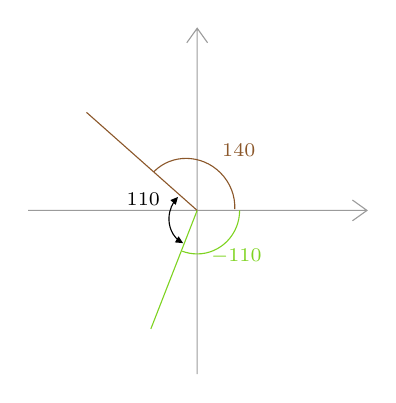
\begin{tikzpicture}[x=0.75pt,y=0.75pt,yscale=-1,xscale=1]
		%uncomment if require: \path (0,300); %set diagram left start at 0, and has height of 300
		
		%Shape: Axis 2D [id:dp8778873795993651] 
		\draw [color={rgb, 255:red, 155; green, 155; blue, 155 }  ,draw opacity=1 ] (138.53,123.78) -- (301.73,123.78)(219.92,36) -- (219.92,202.67) (294.73,118.78) -- (301.73,123.78) -- (294.73,128.78) (214.92,43) -- (219.92,36) -- (224.92,43)  ;
		%Straight Lines [id:da2729508144276438] 
		\draw [color={rgb, 255:red, 139; green, 87; blue, 42 }  ,draw opacity=1 ]   (219.92,123.78) -- (166.6,76.53) ;
		%Straight Lines [id:da7165137837483855] 
		\draw [color={rgb, 255:red, 126; green, 211; blue, 33 }  ,draw opacity=1 ]   (197.6,180.87) -- (219.92,123.78) ;
		%Shape: Arc [id:dp46003831223859915] 
		\draw  [draw opacity=0] (213.14,139.54) .. controls (208.05,137.11) and (205.23,130.85) .. (206.71,124.46) .. controls (207.37,121.59) and (208.8,119.13) .. (210.69,117.29) -- (218.4,127.17) -- cycle ; \draw    (210.62,137.88) .. controls (207.17,134.85) and (205.5,129.7) .. (206.71,124.46) .. controls (207.13,122.66) and (207.85,121.01) .. (208.8,119.58) ; \draw [shift={(210.69,117.29)}, rotate = 131.87] [fill={rgb, 255:red, 0; green, 0; blue, 0 }  ][line width=0.08]  [draw opacity=0] (3.57,-1.72) -- (0,0) -- (3.57,1.72) -- cycle    ; \draw [shift={(213.14,139.54)}, rotate = 210.89] [fill={rgb, 255:red, 0; green, 0; blue, 0 }  ][line width=0.08]  [draw opacity=0] (3.57,-1.72) -- (0,0) -- (3.57,1.72) -- cycle    ;
		%Shape: Arc [id:dp7622599242634296] 
		\draw  [draw opacity=0] (199.12,105.07) .. controls (207.72,96.39) and (222.01,96.61) .. (231.04,105.56) .. controls (235.96,110.43) and (238.3,116.88) .. (238.03,123.15) -- (215.47,121.27) -- cycle ; \draw  [color={rgb, 255:red, 139; green, 87; blue, 42 }  ,draw opacity=1 ] (199.12,105.07) .. controls (207.72,96.39) and (222.01,96.61) .. (231.04,105.56) .. controls (235.96,110.43) and (238.3,116.88) .. (238.03,123.15) ;  
		%Shape: Arc [id:dp05117912063121555] 
		\draw  [draw opacity=0] (240.37,123.78) .. controls (240.37,123.78) and (240.37,123.78) .. (240.37,123.78) .. controls (240.37,135.36) and (231.21,144.74) .. (219.92,144.74) .. controls (217.4,144.74) and (214.99,144.28) .. (212.76,143.43) -- (219.92,123.78) -- cycle ; \draw  [color={rgb, 255:red, 126; green, 211; blue, 33 }  ,draw opacity=1 ] (240.37,123.78) .. controls (240.37,123.78) and (240.37,123.78) .. (240.37,123.78) .. controls (240.37,135.36) and (231.21,144.74) .. (219.92,144.74) .. controls (217.4,144.74) and (214.99,144.28) .. (212.76,143.43) ;  
		
		% Text Node
		\draw (230.73,90.33) node [anchor=north west][inner sep=0.75pt]  [color={rgb, 255:red, 139; green, 87; blue, 42 }  ,opacity=1 ] [align=left] {{\scriptsize $ 140\degree $}};
		% Text Node
		\draw (184.73,114) node [anchor=north west][inner sep=0.75pt]   [align=left] {{\scriptsize $ 110\degree $}};
		% Text Node
		\draw (225.4,141) node [anchor=north west][inner sep=0.75pt]  [color={rgb, 255:red, 126; green, 211; blue, 33 }  ,opacity=1 ] [align=left] {{\scriptsize $ -110\degree $}};
		
		
	\end{tikzpicture}
	
	\caption{Example to show possible misinterpretation of circular data: If \textcolor{brown}{$ \phi_1$}$=140\degree$ and \textcolor{green!70}{$ \phi_2$}$  = -110\degree $, it is easy to see geometrically that $ \Delta\phi= 110\degree $.} 
	\label{fig:example-circ-data}
\end{figure}
%
A common way of visualizing dihedral angles is to make a Ramachandran plot\cite{ramaplot1963}, which is a two-dimensional heatmap of the dihedral angles. After converting the angles to radians, this plot was made here using the built-in \texttt{matplotlib} package \texttt{hist2d}, with 200 bins. The bins were chosen through trial to avoid noisy spikes arising from a higher bin count. A three-dimensional plot of the same was made in figure \ref{fig:ramaplot3d}.

\begin{figure}[htbp]
	\includegraphics[width=0.75\linewidth]{../Coding/final_plots/Rama_plot_initial.pdf}
	\caption{The Ramachandran plot of alanine dipeptide, a two-dimensional probability distribution as a function of $ \phi $ and $ \psi $.}
	\label{fig:ramaplotinitial}
\end{figure}
%
\begin{figure}[htbp]
	\centering
	\includegraphics[width=\linewidth]{../Coding/plots/Rama_plot_3d}
	\caption{3D-projection of the Ramachandran plot made in figure \ref{fig:ramaplotinitial}.}
	\label{fig:ramaplot3d}
\end{figure}
Transforming the distribution to logarithmic scale improved the visibility of the different states observed in the plot (see figure \ref{fig:freeenergyinitial}). Hence the two-dimensional free energy $ \Delta G(\phi,\psi) $ was determined as follows: 
\begin{equation}\label{eq:free-energy-2d}
	\Delta G(\phi, \psi) = -\ln\left(\frac{P(\phi, \psi) + \rho_{\text{min}}}{\rho_{\text{max}}}\right),
\end{equation}
where $ \rho_{\text{min}} $ and  $ \rho_{\text{max}} $ correspond to the minimum and maximum values in the distribution $ P(\phi,\psi) $. The free energy was hence obtained in units of $ k_B T $. The function \texttt{calculate_free_energy} was defined in the notebook to compute the two-dimensional free energy given the probability distribution as a function of two coordinates. This function was used in all four tasks to make the free energy plot.
\begin{figure}
	\centering
	\includegraphics[width=\linewidth]{../Coding/final_plots/free_energy_initial.pdf}
	\caption{The plot of two-dimensional free energy given by equation \ref{eq:free-energy-2d}. Setting the logarithmic scale enhances the visibility of the various regions around the minima, as compared to figure \ref{fig:ramaplotinitial}}
	\label{fig:freeenergyinitial}
\end{figure}
%
%
A simple histogram of the dihedral angles (figure \ref{fig:1dphipsi}) indicate multiple minima positions. The \texttt{bins='auto'} parameter of \texttt{hist2d} can be used to choose the bin count automatically, which gave about 350 bins for $ \phi $ and 150 for $ \psi $. The minima from the 1d distributions were roughly identified on the free energy plot by annotating the plot with vertical and horizontal lines (corresponding to constant $ \phi $ and $ \psi $ values respectively). The points of intersection rightly matched with the observed minima in the Ramachandran plot. The plot also showed that the landscape has a nature of continuity at the boundary (for example, look along the constant $ \phi $ line near $ \phi = \frac{3\pi}{4} $ in figure \ref{fig:freeenergyinitialannotated}). This is another reason to consider a periodic treatment of dihedral angles.

The points of minima in the heatmap (figure \ref{fig:freeenergyinitialannotated}) correspond to different stable conformational states of the dipeptide, since it spends more steps in the trajectory in these states. The distribution of the trajectory indicated that the most stable conformations were the two states in the second quadrant ($ \psi^+ $, $ \phi^- $), which correspond to the $ \beta $ sheet conformation of polypeptides \cite{Richardson1989}. The sharpest peak appeared around the point $ \phi=-10\degree,\,\psi=85\degree $.

\begin{figure*}[htbp]
	\centering
	\includegraphics[width=\linewidth]{../Coding/final_plots/1d_phi_psi.pdf}
	\caption{One-dimensional distributions of $ \phi $ (left) and $ \psi $ (right). The maximas correspond to stable conformational states. $ \phi $ has two major peaks around $ -10\degree $ and $ -80 \degree $, and one minor peak at about $ 120\degree $, while the distribution of $ \psi $ has two major peaks, one around $ -80\degree $ and another at about $ 85\degree $. The distribution is shown here in degrees to easily identify angles.}
	\label{fig:1dphipsi}
\end{figure*}
\begin{figure}[htbp]
	\centering
	\includegraphics[width=\linewidth]{../Coding/final_plots/free_energy_initial_annotated.pdf}
	\caption{Free energy landscape annotated with rough estimates of minima obtained from figure \ref{fig:1dphipsi}.}
	\label{fig:freeenergyinitialannotated}
\end{figure}
%
%\begin{equation}\label{eq:free-energy}
%	F(\xi) \propto -\ln P(\xi),	
%\end{equation}
%
%where $ \xi \in \{\phi,\psi\} $. For the calculation, a small value \texttt{epsilon} is added within the argument of the \texttt{log} function in Python, to avoid getting infinity. The obtained distributions of the free energies are shown in figure \ref{fig:freeenergyprojectionssubplots}.

\subsection{Task II: Principal Component Analysis (PCA)}\label{ssec:task2_pca}
%
The trajectory of the dipeptide molecule were imported as two arrays:
\begin{equation}\label{eq:phi-psi-vector}
	\phi = \begin{pmatrix}
		\phi_1\\
		\phi_2\\
		\vdots\\
		\phi_N
	\end{pmatrix} \qquad \psi = \begin{pmatrix}
		\psi_1\\
		\psi_2\\
		\vdots\\
		\psi_N
	\end{pmatrix}
\end{equation}
The first task in the project was to perform a regular PCA of the variables given. The covariance between the variables is defined as
\begin{equation}\label{eq:covariance}
	\Cov{\phi,\psi} = \frac{1}{N} \sum_{i=1}^{N} \left( \phi - \expval{\phi} \right)\left( \psi - \expval{\psi} \right),
\end{equation}
and the variance of each variable
\begin{equation}\label{eq:variance}
	\Var{\xi} = \Cov{\xi,\xi} = \frac{1}{N} \sum_{i=1}^{N} \left( \xi - \expval{\xi} \right)^2
\end{equation}
with $ \xi \in \{\phi,\psi\} $. The covariance matrix is defined with these two quantities as elements:
\begin{equation}\label{eq:cov-matrix}
	C = \begin{pmatrix}
		\Var{\phi}& \Cov{\phi,\psi}\\
		\Cov{\phi,\psi}& \Var{\psi}
	\end{pmatrix}
\end{equation}
The covariance matrix was computed using the \texttt{numpy} method \texttt{cov(arr1,arr2)}, where \texttt{arr1} and \texttt{arr2} are the arrays whose covariance is studied. %The obtained covariance matrix is:
%\begin{equation}\label{eq:cov-matrix-vals}
%	C = \begin{pmatrix}
	%		0.49& -0.15\\
	%		-0.15&	1.8
	%	\end{pmatrix}
%\end{equation}
%%
Diagonalizing the matrix, the eigenvalues ($ \lambda_1 $, $ \lambda_2 $) and eigenvectors $ \vec{e}_1, $ $\vec{e}_2$ $ $ were computed. The eigenvector corresponding to the higher eigenvalue of the two is the principal component 1 (PC 1), a unit vector. After centering the data by subtracting the mean value, the data points were projected along the principal components, by taking a dot-product. 
\begin{equation}\label{eq:projection-dot}
	\left( \vec{e}_0, \vec{e}_1 \right)^T \cdot \left( \phi(t), \psi(t) \right)^{T} = \left( V_1 (t), V_2 (t) \right)^T
\end{equation}
Finally, the free energy and the one-dimensional distributions of the data projected (labeled $ V_1 $ and $ V_2 $) were plotted (figures \ref{fig:freeenergypca} and \ref{fig:1dv1v2} respectively). 
%
\subsection{Task III: dPCA}\label{ssec:task3_dpca}
%
To linearize the (periodic) data, the sine and cosine transformations of the dihedral angles were computed, thereby getting four arrays. The PCA (or more precisely, dPCA) was performed on the four new variables $ \sin\phi,\cos\phi,\sin\psi $ and $ \cos\psi $. The arrays of these four variables were stacked into a single variable \texttt{stacked_arr} (of order $ 4\times N $) to compute the covariance matrix. The covariance matrix (equation \ref{eq:cov-matrix}) in this case was a $ 4\times 4 $ matrix, compared to the PCA, where the matrix had order $ 2\times 2 $. The elements of this covariance matrix can be explicitly written down as in equation \ref{eq:cov-matrix-dPCA}.
\begin{table*}
	\begin{equation}\label{eq:cov-matrix-dPCA}
		C_{\text{dPCA}} = \begin{pmatrix}
			\Var{\sin(\phi)} & \Cov{\sin(\phi),\cos(\phi)} & \Cov{\sin(\phi),\sin(\psi)} & \Cov{\sin(\phi),\cos(\psi)} \\
			\Cov{\cos(\phi),\sin(\phi)} & \Var{\cos(\phi)} & \Cov{\cos(\phi),\sin(\psi)} & \Cov{\cos(\phi),\cos(\psi)} \\
			\Cov{\sin(\psi),\sin(\phi)} & \Cov{\sin(\psi),\cos(\phi)} & \Var{\sin(\psi)} & \Cov{\sin(\psi),\cos(\psi)} \\
			\Cov{\cos(\psi),\sin(\phi)} & \Cov{\cos(\psi),\cos(\phi)} & \Cov{\cos(\psi),\sin(\psi)} & \Var{\cos(\psi)}
		\end{pmatrix}
	\end{equation}
\end{table*}

The four obtained eigenvectors were arranged in decreasing order, and the principal components were identified. Following the guidelines of the given task, the data was projected only to the first two principal components. A scree plot, the free energy and one-dimensional distributions were plotted for the resulting components.
%
\begin{figure*}[htbp]
	\centering
	\includegraphics[width=\linewidth]{../Coding/final_plots/1d_dPCA_V1_V2}
	\caption{The one-dimensional projections of the first two PCs obtained as a result of dPCA.}
	\label{fig:1d-dpcav1v2}
\end{figure*}
%
%
%
\subsection{Task IV: dPCA+}\label{ssec:task4_dpcaPlus}
%
As given in the task description, the maximal gap in the histogram were defined by minimizing the point density of a corridor as follows. For a bin size of 150, the two-dimensional histogram of the free energy along both dihedral angles is plotted. This plot was chosen over the regular Ramachandran plot because the latter only showed points of high concentration, so the choice of a maximal gap would be too broad to choose from. The maximal gap was identified in three stages:
\begin{enumerate}
	\item 	As a starting point, a visual estimate of a potential cut point for $ \phi $ was made. A line at the estimated point was plotted in the 2D free energy plot (vertical line corresponding to constant $ \phi $ value, and horizontal line corresponding to constant $ \psi $). 
	\item 	This cut point was fine-tuned by following a kind of bisection method successively. For example, if one low point-density corridor was identified between $ \phi $-values $ \nicefrac{\pi}{4} $ and $ \nicefrac{\pi}{2} $, a constant $ \phi $ line was made at their mean position, \textit{i.e.,} at $\phi= \nicefrac{3\pi}{8} $. The initial guessed line was then shifted to this position to see if it could be further improved. After two iterations, a $ \phi $ value of $ \nicefrac{11\pi}{32} $ was finalized to be the first guess (figure \ref{fig:freeenergymaxgap}). The estimated positions were also visualized in the one-dimensional projections (Note that at this point, this value is still a \textit{guess}). 
	\item 	To fine-tune the above choice, a function \texttt{find_best_maximal_gap} was defined to perform a search for the bins with the least number of counts in the neighbourhood of the guessed value. On inputting the histogram data, this function identifies the best bin to shift the data. The numpy function \texttt{searchsorted} is utilized for this purpose\footnote{The \texttt{searchsorted} function here takes a sorted array (\texttt{bin_edges} in this case) and a value (\texttt{guess_value}) and returns the index at which this value should be inserted to maintain the order of the array.}. The values returned by this search function is finalized for further analysis. 
\end{enumerate}
The initial guess and optimized values (called $ \phi_0 $ and $ \psi_0 $ from here onward) are shown in the free energy plot in figure \ref{fig:freeenergymaxgapbest}. The angles were shifted by defining the function \texttt{shift_angles}. Hence the range of the data was transformed as equation \ref{eq:PBC-shift-2}.
\begin{figure*}[htbp]
	\begin{equation}
		\label{eq:PBC-shift-2}
		\left[-\pi, \pi \right) \times \left[-\pi, \pi \right) \mapsto \left[-\pi + \phi_{\text{offset}}, \pi + \phi_{\text{offset}} \right) \times \left[-\pi + \psi_{\text{offset}}, \pi + \psi_{\text{offset}} \right)
	\end{equation}
\end{figure*}
\begin{figure}[htbp]
	\centering
	\includegraphics[width=\linewidth]{../Coding/final_plots/free_energy_max_gap_best}
	\caption{Identifying the maximal gap window. After an initial visual guess (dotted lines), the \texttt{find_best_maximal_gap} function optimizes this choice by a search (optimized position in continuous red line). The final cut points are $ \phi_0 \approx 52.8\degree $ and $ \psi_0 \approx -172.3 \degree $.}
	\label{fig:freeenergymaxgapbest}
\end{figure}
%
\begin{figure*}[htp]
	\centering
	\begin{subfigure}[b]{0.45\textwidth}
		\centering
		\includegraphics[width=\textwidth]{../Coding/final_plots/shifting_PB_phi.pdf}
		\caption{Original and shifted distributions for $ \phi $}
		\label{fig:shifted_phi}
	\end{subfigure}
	\hfill
	\begin{subfigure}[b]{0.45\textwidth}
		\centering
		\includegraphics[width=\textwidth]{../Coding/final_plots/shifting_PB_psi.pdf}
		\caption{Original and shifted distributions for $ \psi $}
		\label{fig:shifted_psi}
	\end{subfigure}
	\caption{Shifted angles for $ \phi $ and $ \psi $}
	\label{fig:shifted_angles}
\end{figure*}
%
\begin{figure}[htbp]
	\centering
	\includegraphics[width=\linewidth]{../Coding/final_plots/free_energy_max_gap.pdf}
	\caption{Initial (visual) guess for the maximal gap}
	\label{fig:freeenergymaxgap}
\end{figure}
%
Using the new shifted distributions of $ \phi $ and $ \psi $, a PCA is performed with these variables, and associated plots made, just as in the previous tasks.